\chapter[Matrici e Sistemi]{Matrici e Sistemi Lineari}
\label{ch:matrici-sistemi}

Le matrici sono lo strumento computazionale fondamentale dell'algebra lineare. In questo capitolo introduciamo le operazioni su matrici e le utilizziamo per risolvere sistemi di equazioni lineari tramite il metodo di eliminazione di Gauss.

\section{Matrici: definizioni e operazioni}
\label{sec:matrici-def}

\begin{definitionbox}[Matrice]
Una \textbf{matrice} $A$ di tipo $m \times n$ a coefficienti in $\mathbb{R}$ è una tabella rettangolare di $m$ righe e $n$ colonne:
\[ A = \begin{pmatrix} a_{11} & a_{12} & \cdots & a_{1n} \\ a_{21} & a_{22} & \cdots & a_{2n} \\ \vdots & \vdots & \ddots & \vdots \\ a_{m1} & a_{m2} & \cdots & a_{mn} \end{pmatrix} \in \mathcal{M}_{m \times n}(\mathbb{R}). \]
L'elemento $a_{ij}$ si trova nella riga $i$ e nella colonna $j$. Scriviamo anche $A = (a_{ij})$.
\end{definitionbox}

\begin{definitionbox}[Operazioni su matrici]
Date $A, B \in \mathcal{M}_{m \times n}(\mathbb{R})$ e $\lambda \in \mathbb{R}$:
\begin{itemize}
    \item \textbf{Somma}: $(A + B)_{ij} = a_{ij} + b_{ij}$
    \item \textbf{Prodotto per scalare}: $(\lambda A)_{ij} = \lambda \, a_{ij}$
\end{itemize}
Con queste operazioni, $\mathcal{M}_{m \times n}(\mathbb{R})$ è uno spazio vettoriale di dimensione $mn$.
\end{definitionbox}

\begin{definitionbox}[Prodotto righe per colonne]
\label{def:prodotto-matrici}
Date $A \in \mathcal{M}_{m \times p}(\mathbb{R})$ e $B \in \mathcal{M}_{p \times n}(\mathbb{R})$, il \textbf{prodotto} $C = AB \in \mathcal{M}_{m \times n}(\mathbb{R})$ è definito da:
\[ c_{ij} = \sum_{k=1}^{p} a_{ik} \, b_{kj} \quad \text{per ogni } i = 1, \ldots, m, \; j = 1, \ldots, n. \]
\end{definitionbox}

\begin{notebox}[Il prodotto non è commutativo]
In generale $AB \neq BA$, anche quando entrambi i prodotti sono definiti. Ad esempio, per matrici $2 \times 2$:
\[ A = \begin{pmatrix} 1 & 0 \\ 0 & 0 \end{pmatrix}, \quad B = \begin{pmatrix} 0 & 1 \\ 0 & 0 \end{pmatrix} \quad \Longrightarrow \quad AB = \begin{pmatrix} 0 & 1 \\ 0 & 0 \end{pmatrix}, \quad BA = \begin{pmatrix} 0 & 0 \\ 0 & 0 \end{pmatrix}. \]
\end{notebox}

\begin{examplebox}[Prodotto di matrici]
Calcoliamo il prodotto:
\[ \begin{pmatrix} 1 & 2 \\ 3 & 4 \end{pmatrix} \begin{pmatrix} 5 & 6 \\ 7 & 8 \end{pmatrix} = \begin{pmatrix} 1 \cdot 5 + 2 \cdot 7 & 1 \cdot 6 + 2 \cdot 8 \\ 3 \cdot 5 + 4 \cdot 7 & 3 \cdot 6 + 4 \cdot 8 \end{pmatrix} = \begin{pmatrix} 19 & 22 \\ 43 & 50 \end{pmatrix}. \]
\end{examplebox}

\begin{definitionbox}[Matrici particolari]
\begin{itemize}
    \item \textbf{Matrice identità}: $I_n = (\delta_{ij})$ dove $\delta_{ij}$ è il delta di Kronecker. Vale $AI_n = I_m A = A$.
    \item \textbf{Matrice trasposta}: $(A^T)_{ij} = a_{ji}$. Valgono $(AB)^T = B^T A^T$ e $(A^T)^T = A$.
    \item \textbf{Matrice inversa}: $A \in \mathcal{M}_{n \times n}(\mathbb{R})$ è \textbf{invertibile} se esiste $A^{-1}$ tale che $AA^{-1} = A^{-1}A = I_n$.
    \item \textbf{Matrice simmetrica}: $A = A^T$, cioè $a_{ij} = a_{ji}$ per ogni $i, j$.
\end{itemize}
\end{definitionbox}

\begin{theorembox}[Proprietà dell'inversa]
Sia $A$ una matrice quadrata invertibile. Allora:
\begin{enumerate}
    \item $A^{-1}$ è unica.
    \item $(A^{-1})^{-1} = A$.
    \item $(AB)^{-1} = B^{-1}A^{-1}$ (se $B$ è invertibile).
    \item $(A^T)^{-1} = (A^{-1})^T$.
\end{enumerate}
\end{theorembox}

\section{Sistemi di equazioni lineari}
\label{sec:sistemi-lineari}

\begin{definitionbox}[Sistema lineare]
Un \textbf{sistema di $m$ equazioni lineari in $n$ incognite} è:
\[
\begin{cases}
a_{11}x_1 + a_{12}x_2 + \cdots + a_{1n}x_n = b_1 \\
a_{21}x_1 + a_{22}x_2 + \cdots + a_{2n}x_n = b_2 \\
\quad \vdots \\
a_{m1}x_1 + a_{m2}x_2 + \cdots + a_{mn}x_n = b_m
\end{cases}
\]
In forma matriciale si scrive $A\mathbf{x} = \mathbf{b}$, dove $A \in \mathcal{M}_{m \times n}(\mathbb{R})$ è la \textbf{matrice dei coefficienti}, $\mathbf{x} \in \mathbb{R}^n$ è il vettore delle incognite e $\mathbf{b} \in \mathbb{R}^m$ è il vettore dei termini noti.
\end{definitionbox}

\begin{definitionbox}[Matrice completa]
La \textbf{matrice completa} (o aumentata) del sistema è:
\[ (A \mid \mathbf{b}) = \left( \begin{array}{cccc|c} a_{11} & a_{12} & \cdots & a_{1n} & b_1 \\ a_{21} & a_{22} & \cdots & a_{2n} & b_2 \\ \vdots & \vdots & \ddots & \vdots & \vdots \\ a_{m1} & a_{m2} & \cdots & a_{mn} & b_m \end{array} \right). \]
Il sistema è \textbf{omogeneo} se $\mathbf{b} = \mathbf{0}$.
\end{definitionbox}

\begin{figure}[htbp]
  \centering
  
\includegraphics[width=0.85\textwidth]{ch02-systems-geometry}
  \caption{Interpretazione geometrica di un sistema lineare di tre equazioni in tre incognite: soluzione unica (intersezione in un punto), infinite soluzioni (intersezione lungo una retta), nessuna soluzione (piani senza punti comuni).}
  \label{fig:ch02-systems-geometry}
\end{figure}

\section{Eliminazione di Gauss}
\label{sec:gauss}

L'idea del metodo di Gauss è trasformare la matrice completa in una forma ``a scalini'' tramite operazioni elementari che non cambiano le soluzioni.

\begin{definitionbox}[Operazioni elementari sulle righe]
Le operazioni elementari su una matrice sono:
\begin{enumerate}
    \item $R_i \leftrightarrow R_j$: scambiare due righe;
    \item $R_i \to \lambda R_i$ con $\lambda \neq 0$: moltiplicare una riga per uno scalare non nullo;
    \item $R_i \to R_i + \lambda R_j$: sommare a una riga un multiplo di un'altra.
\end{enumerate}
Due matrici legate da operazioni elementari si dicono \textbf{equivalenti per righe}.
\end{definitionbox}

\begin{definitionbox}[Forma a scalini]
Una matrice è in \textbf{forma a scalini} (per righe) se:
\begin{enumerate}
    \item Le eventuali righe nulle sono in fondo.
    \item Il primo elemento non nullo di ogni riga (detto \textbf{pivot}) si trova a destra del pivot della riga precedente.
\end{enumerate}
Se inoltre ogni pivot vale $1$ e è l'unico elemento non nullo nella sua colonna, la matrice è in \textbf{forma a scalini ridotta} (di Gauss--Jordan).
\end{definitionbox}

\begin{examplebox}[Eliminazione di Gauss]
\label{ex:gauss}
Risolviamo il sistema:
\[
\begin{cases}
x + 2y - z = 3 \\
2x + 5y + z = 8 \\
x + 3y + 2z = 5
\end{cases}
\]
Scriviamo la matrice completa e riduciamo a scalini:
\[
\left( \begin{array}{ccc|c} 1 & 2 & -1 & 3 \\ 2 & 5 & 1 & 8 \\ 1 & 3 & 2 & 5 \end{array} \right)
\xrightarrow[\scriptscriptstyle R_3 - R_1]{\scriptscriptstyle R_2 - 2R_1}
\left( \begin{array}{ccc|c} 1 & 2 & -1 & 3 \\ 0 & 1 & 3 & 2 \\ 0 & 1 & 3 & 2 \end{array} \right)
\]
\[
\xrightarrow{\scriptscriptstyle R_3 - R_2}
\left( \begin{array}{ccc|c} 1 & 2 & -1 & 3 \\ 0 & 1 & 3 & 2 \\ 0 & 0 & 0 & 0 \end{array} \right)
\]
La variabile $z$ è libera. Dalla seconda riga: $y = 2 - 3z$. Dalla prima: $x = 3 - 2(2-3z) + z = -1 + 7z$. Le soluzioni sono:
\[ (x, y, z) = (-1 + 7t, \; 2 - 3t, \; t), \quad t \in \mathbb{R}. \]
\end{examplebox}

\section{Rango di una matrice}
\label{sec:rango}

\begin{definitionbox}[Rango]
Il \textbf{rango} di una matrice $A$, indicato con $\text{rk}(A)$ o $\text{rg}(A)$, è il numero di pivot nella sua forma a scalini, equivalentemente:
\begin{itemize}
    \item Il massimo numero di righe linearmente indipendenti di $A$.
    \item Il massimo numero di colonne linearmente indipendenti di $A$.
    \item La dimensione dello spazio generato dalle colonne di $A$ (spazio colonna).
\end{itemize}
\end{definitionbox}

\begin{theorembox}[Proprietà del rango]
Per ogni $A \in \mathcal{M}_{m \times n}(\mathbb{R})$:
\begin{enumerate}
    \item $0 \leq \text{rk}(A) \leq \min(m, n)$.
    \item $\text{rk}(A) = \text{rk}(A^T)$.
    \item $\text{rk}(AB) \leq \min(\text{rk}(A), \text{rk}(B))$.
    \item Se $A$ è quadrata $n \times n$: $A$ è invertibile $\Leftrightarrow$ $\text{rk}(A) = n$.
\end{enumerate}
\end{theorembox}

\begin{examplebox}[Calcolo del rango]
\[ A = \begin{pmatrix} 1 & 2 & 3 \\ 2 & 4 & 6 \\ 0 & 1 & 1 \end{pmatrix} \xrightarrow{R_2 \to R_2 - 2R_1} \begin{pmatrix} 1 & 2 & 3 \\ 0 & 0 & 0 \\ 0 & 1 & 1 \end{pmatrix} \xrightarrow{R_2 \leftrightarrow R_3} \begin{pmatrix} 1 & 2 & 3 \\ 0 & 1 & 1 \\ 0 & 0 & 0 \end{pmatrix} \]
La forma a scalini ha $2$ pivot, quindi $\text{rk}(A) = 2$.
\end{examplebox}

\section[Rouch\'e--Capelli]{Teorema di Rouch\'e--Capelli}
\label{sec:rouche-capelli}

\begin{theorembox}[Teorema di Rouch\'e--Capelli]
\label{thm:rouche-capelli}
Il sistema $A\mathbf{x} = \mathbf{b}$ ammette soluzioni se e solo se:
\[ \text{rk}(A) = \text{rk}(A \mid \mathbf{b}). \]
In tal caso, se $A \in \mathcal{M}_{m \times n}(\mathbb{R})$ e $\text{rk}(A) = r$, l'insieme delle soluzioni è un sottospazio affine di $\mathbb{R}^n$ di dimensione $n - r$ (le variabili libere sono $n - r$).
\end{theorembox}

\begin{notebox}[Conseguenze importanti]
\begin{itemize}
    \item Se $\text{rk}(A) = \text{rk}(A \mid \mathbf{b}) = n$ (numero di incognite): la soluzione è \textbf{unica}.
    \item Se $\text{rk}(A) = \text{rk}(A \mid \mathbf{b}) < n$: ci sono $\infty^{n-r}$ soluzioni.
    \item Se $\text{rk}(A) < \text{rk}(A \mid \mathbf{b})$: il sistema è \textbf{impossibile}.
\end{itemize}
\end{notebox}

\begin{theorembox}[Struttura delle soluzioni]
\label{thm:struttura-soluzioni}
Se il sistema $A\mathbf{x} = \mathbf{b}$ è compatibile e $\mathbf{x}_0$ è una soluzione particolare, allora l'insieme di tutte le soluzioni è:
\[ \mathcal{S} = \{\mathbf{x}_0 + \mathbf{v} : \mathbf{v} \in \ker(A)\} = \mathbf{x}_0 + \ker(A) \]
dove $\ker(A) = \{\mathbf{v} \in \mathbb{R}^n : A\mathbf{v} = \mathbf{0}\}$ è l'insieme delle soluzioni del sistema omogeneo associato.
\end{theorembox}

\begin{examplebox}[Applicazione del teorema di Rouch\'e--Capelli]
Determiniamo per quali valori di $k \in \mathbb{R}$ il sistema seguente è compatibile:
\[
\begin{cases}
x + y + z = 1 \\
2x + y - z = 0 \\
3x + 2y = k
\end{cases}
\]
La matrice completa è:
\[ (A \mid \mathbf{b}) = \left( \begin{array}{ccc|c} 1 & 1 & 1 & 1 \\ 2 & 1 & -1 & 0 \\ 3 & 2 & 0 & k \end{array} \right) \xrightarrow[\scriptscriptstyle R_3 - 3R_1]{\scriptscriptstyle R_2 - 2R_1} \left( \begin{array}{ccc|c} 1 & 1 & 1 & 1 \\ 0 & -1 & -3 & -2 \\ 0 & -1 & -3 & k{-}3 \end{array} \right) \]
\[ \xrightarrow{R_3 \to R_3 - R_2} \left( \begin{array}{ccc|c} 1 & 1 & 1 & 1 \\ 0 & -1 & -3 & -2 \\ 0 & 0 & 0 & k-1 \end{array} \right) \]
Se $k \neq 1$: $\text{rk}(A) = 2 < 3 = \text{rk}(A \mid \mathbf{b})$, il sistema è \textbf{impossibile}.

Se $k = 1$: $\text{rk}(A) = \text{rk}(A \mid \mathbf{b}) = 2$, con $3 - 2 = 1$ variabile libera. Le soluzioni sono:
\[ (x, y, z) = (-1 + 2t, \; 2 - 3t, \; t), \quad t \in \mathbb{R}. \]
\end{examplebox}

\begin{figure}[htbp]
\centering
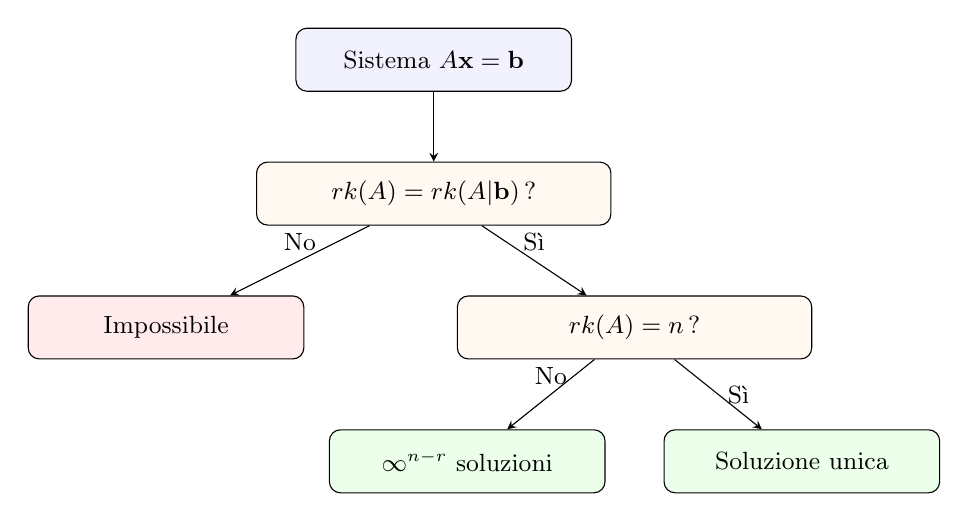
\begin{tikzpicture}[>=stealth, scale=0.85,
    block/.style={draw, rounded corners, minimum width=3.5cm, minimum height=0.8cm, font=\small},
    decision/.style={draw, rounded corners, fill=orange!5, minimum width=4.5cm, minimum height=0.8cm, font=\small}]
    \node[block, fill=blue!5] (start) at (0,0) {Sistema $A\mathbf{x} = \mathbf{b}$};
    \node[decision] (check) at (0,-2) {$\text{rk}(A) = \text{rk}(A|\mathbf{b})$\,?};
    \node[block, fill=red!8] (no) at (-4,-4) {Impossibile};
    \node[decision] (check2) at (3,-4) {$\text{rk}(A) = n$\,?};
    \node[block, fill=green!8] (unique) at (5.5,-6) {Soluzione unica};
    \node[block, fill=green!8] (inf) at (0.5,-6) {$\infty^{n-r}$ soluzioni};

    \draw[->] (start) -- (check);
    \draw[->] (check) -- node[above] {\small No} (no);
    \draw[->] (check) -- node[above] {\small Sì} (check2);
    \draw[->] (check2) -- node[right] {\small Sì} (unique);
    \draw[->] (check2) -- node[above] {\small No} (inf);
\end{tikzpicture}
\caption{Schema decisionale per la compatibilità di un sistema lineare.}
\label{fig:schema-sistema}
\end{figure}

\begin{notebox}[Riepilogo del capitolo]
In questo capitolo abbiamo introdotto:
\begin{itemize}
    \item Le \textbf{matrici} e le loro operazioni (somma, prodotto, trasposta, inversa).
    \item I \textbf{sistemi lineari} e la loro rappresentazione matriciale.
    \item Il \textbf{metodo di Gauss} per la riduzione a scalini.
    \item Il \textbf{rango} come numero di pivot e misura dell'``informazione'' contenuta nella matrice.
    \item Il \textbf{teorema di Rouché--Capelli} come criterio di compatibilità.
\end{itemize}
Nel prossimo capitolo studieremo i \textbf{determinanti}, che forniscono un criterio algebrico per l'invertibilità.
\end{notebox}
